\documentclass[border=3]{standalone}
\usepackage{tikz}
\usepackage{tkz-euclide}

\begin{document}
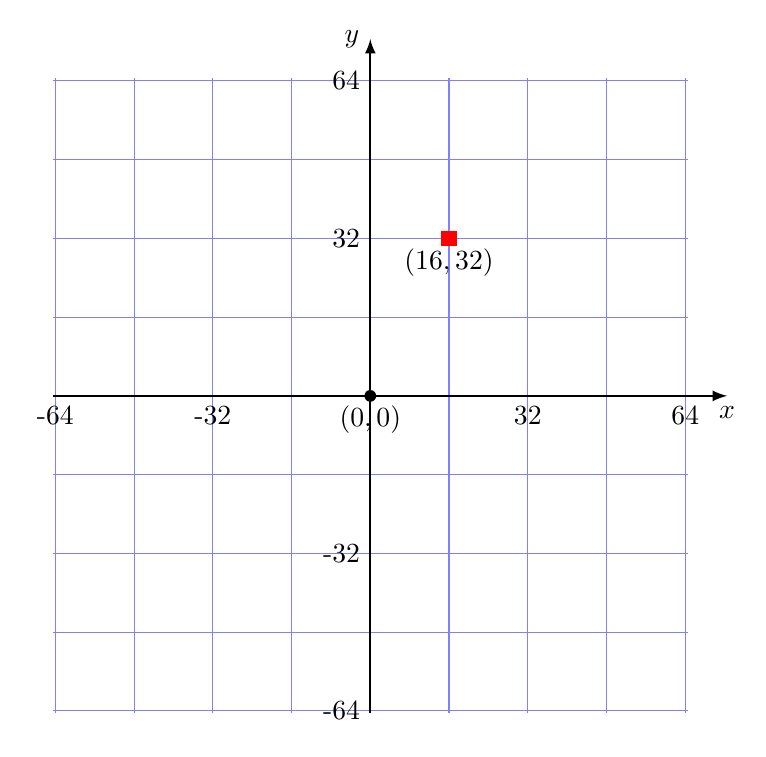
\begin{tikzpicture}
  \tkzInit[xmin=-64.5,xstep=16,xmax=64.5, ymin=-64.5, ystep=16,ymax=64.5]
  \tkzGrid[color=blue!50!white]
  \tkzDrawX[thick,>=latex,label=$x$]
  \tkzDrawY[thick,>=latex,label=$y$]

  \foreach \x in {-64,-32,32,64}
  { \tkzDefPoint(\x,0){$\x$}
    \tkzLabelPoints[below]($\x$) }

  \foreach \y in {-64,-32,32,64}
  { \tkzDefPoint(0,\y){$\y$}
    \tkzLabelPoints[left]($\y$) }

  \tkzDefPoint(0,0){O}
  \tkzLabelPoint[](O){$(0,0)$}
  \node at (O)[circle,fill,inner sep=1.5pt]{};

  \tkzDefPoint(16,32){A}
  \node at (A)[rectangle,fill=red,inner sep=1.5pt, minimum size=0.2cm]{};
  \tkzLabelPoint[](A){$(16,32)$}

  %\draw[draw=black] (16,32) rectangle ++(1,1);
\end{tikzpicture}
\end{document}
